\documentclass[conference]{IEEEtran}
\IEEEoverridecommandlockouts
% The preceding line is only needed to identify funding in the first footnote. If that is unneeded, please comment it out.
\usepackage{cite}
\usepackage{amsmath,amssymb,amsfonts}
\usepackage{algorithmic}
\usepackage{graphicx}
\usepackage{textcomp}
\usepackage{xcolor}
\usepackage{tabularx}
\usepackage{multirow}
\usepackage{graphics} % for pdf, bitmapped graphics files
\usepackage{subfig}
\usepackage{subcaption}
\usepackage{hyperref}
\usepackage{academicons}
\usepackage{xcolor}
\usepackage{listings}
\usepackage{tabularx} % Asegúrate de incluir este paquete

\usepackage{tikz}
\usetikzlibrary{shapes.geometric, arrows}

\usetikzlibrary{shapes.geometric, arrows}

\tikzstyle{startstop} = [rectangle, rounded corners, minimum width=3cm, minimum height=1cm,text centered, draw=black, fill=red!30]
\tikzstyle{process} = [rectangle, minimum width=3cm, minimum height=1cm, text centered, draw=black, fill=blue!30]
\tikzstyle{arrow} = [thick,->,>=stealth]


\def\BibTeX{{\rm B\kern-.05em{\sc i\kern-.025em b}\kern-.08em
		T\kern-.1667em\lower.7ex\hbox{E}\kern-.125emX}}

% Color Enlace
\definecolor{colorEnlace}{RGB}{0, 0, 0}
\hypersetup{
	colorlinks=true,
	linkcolor=colorEnlace,
	citecolor=colorEnlace,
	urlcolor=colorEnlace,
	pdfauthor={Davis Bremdow Salazar Roa},
	pdftitle={Sistemas Embebidos}
}
\definecolor{mybg}{rgb}{0.97,0.97,0.97}
\definecolor{mygray}{gray}{0.4}
\definecolor{mygreen}{rgb}{0,0.6,0}
\definecolor{myblue}{rgb}{0,0,0.8}
\definecolor{mypurple}{rgb}{0.58,0,0.82}
\definecolor{myred}{rgb}{0.7,0,0}

\lstdefinelanguage{MatlabEnhanced}{
	language=Matlab,
	morekeywords={[2]linspace,plot,title,xlabel,ylabel,legend,grid},
	morekeywords={[3]sin,cos,exp,log,sqrt},
	keywordstyle=\color{myblue}\bfseries,
	keywordstyle=[2]\color{mypurple},
	keywordstyle=[3]\color{myred},
	commentstyle=\color{mygreen}\itshape,
	stringstyle=\color{mygray},
	morecomment=[l]%
}

\lstset{
	language=MatlabEnhanced,
	backgroundcolor=\color{mybg},
	frame=single,
	basicstyle=\ttfamily\small,
	showstringspaces=false,
	numbers=none,              %
	xleftmargin=0pt,           %
	framexleftmargin=0pt,      
	framexrightmargin=0pt,
	framextopmargin=2pt,
	framexbottommargin=2pt,
	breaklines=true,
	tabsize=1,
}

% Control 
\usepackage{amsmath}
\begin{document}
	
	\title{Análisis del flujo, presión y volumen en respiradores mecánicos}
	\author{
		\makebox[\textwidth][c]{\large\textbf{Universidad Nacional de San Antonio Abad del Cusco}}\\
		\makebox[\textwidth][c]{\normalsize\textit{Escuela profesional de Ingeniería Electrónica}}\\
		\makebox[\textwidth][c]{\normalsize\textit{Fundamentos de Bioingenieria}}\\
		\and
		\IEEEauthorblockN{Ing. Luis Jimenez Troncoso}
		\IEEEauthorblockA{Ingeniero Electrónico \\
			Cusco, Perú \\
			luis.jimenez@unsaac.edu.pe}
		\and
		\IEEEauthorblockN{Davis Bremdow Salazar Roa - 200353}
		\IEEEauthorblockA{Estudiante de Ingeniería Electrónica \\
			Cusco, Perú \\
			200353@unsaac.edu.pe
		}
	}
	
	\maketitle
	\begin{abstract}
		
	\end{abstract}
	
	\begin{IEEEkeywords}
		
	\end{IEEEkeywords}
	
	%% Contenido del documento
	\section{Obtención del flujo en mL/s a partir de las mediciones de voltaje}
	
	Para el procesamiento de los datos se hizo uso del entorno de MATLAB, utilizando para la carga de los datos el periodo de muestreo con el archivo de texto para las mediciones de flujo en forma de voltaje.
	
	\begin{figure}[h]
		\centering
		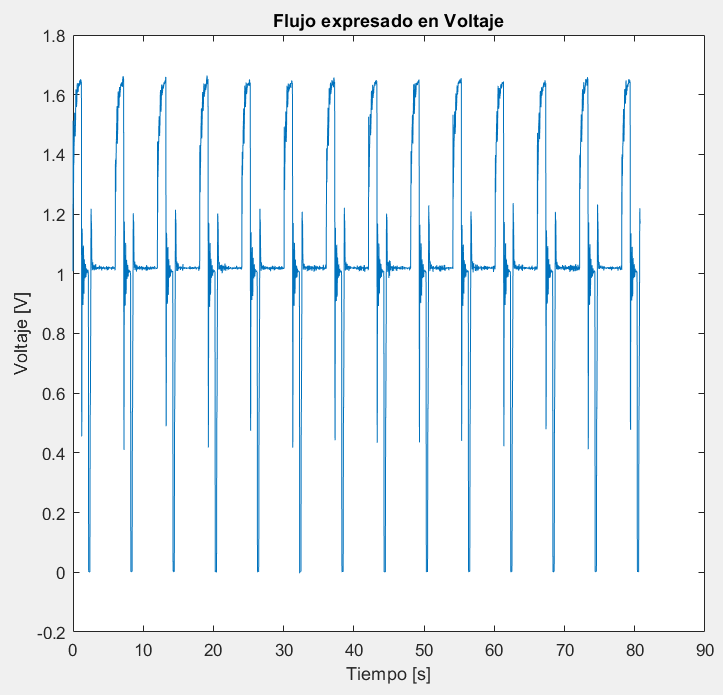
\includegraphics[width=0.35\textwidth]{./media/flujo-voltaje}
		\caption{Forma de onda del flujo expresado en forma de voltaje}
		\label{fig:flujo-voltaje}
	\end{figure}
	
	En la figura \ref{fig:flujo-voltaje} se muestra la gráfica de los datos crudos o sin procesar del flujo - voltaje respecto al tiempo medido en segundos.
	
	Para encontrar la relación entre el flujo en [L/min] es necesario hacer uso de la curva de calibración para el dispositivo, esta se puede encontrar en el manual de uso u hoja de datos del sensor de flujo, siendo para este caso el empleo de la curva perteneciente al D6F-20A que se muestra en la figura \ref{fig:calibracion-flujo}
	
	\begin{figure}[h]
		\centering
		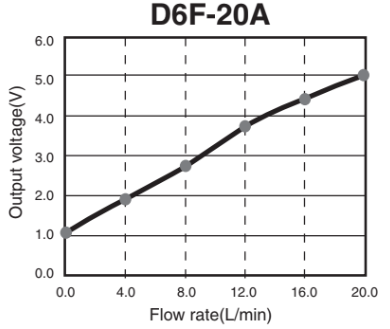
\includegraphics[width=0.3\textwidth]{media/calibracion-flujo}
		\caption{Curva Voltaje [V] - Flujo [L/min}
		\label{fig:calibracion-flujo}
	\end{figure}
	
	Una aproximación más cercana o precisa también se puede realizar mediante el empleo de los valores de flujo y voltaje tabulados también en la hoja de datos.
	
	Por otro lado para la obtención de la curva de calibración se tomaron 2 puntos de la curva mostrada en la figura \ref{fig:calibracion-flujo} para obtener la ecuación de la recta aproximada y la cual se define en \ref{eq:calibracion-flujo}
	
	\begin{equation}
		F = 5(V-1)
		\label{eq:calibracion-flujo}
	\end{equation}
	
	Finalmente una vez obtenido el flujo en este caso en [L/min] se multiplican estos valores por un factor de conversión de 1000/60 para obtener el resultado en [mL/s], según lo especificado, mostrado en la figura \ref{fig:flujo}
	
	\begin{figure}[h]
		\centering
		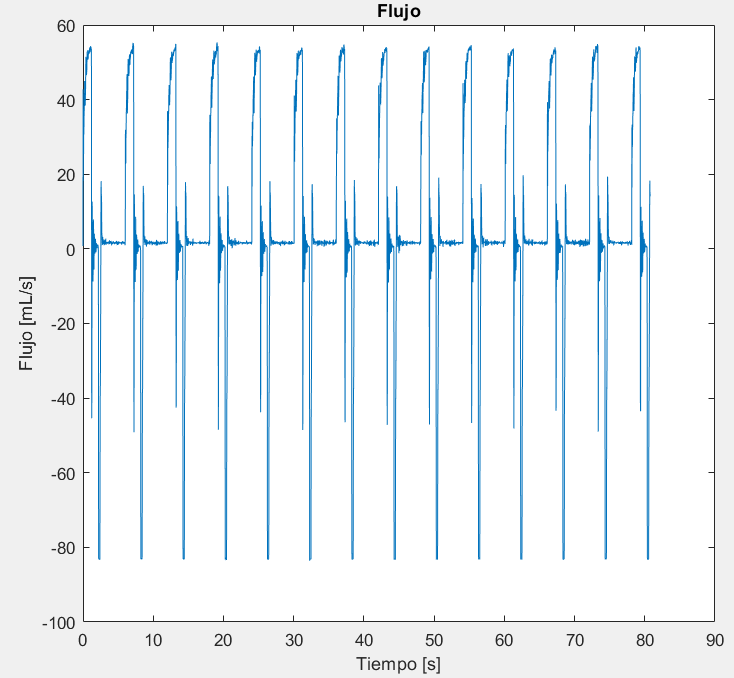
\includegraphics[width=0.4\textwidth]{media/flujo}
		\caption{Curva del Flujo expresada en mL/s}
		\label{fig:flujo}
	\end{figure}
	
	\section{Obtención de la presión en cm Agua a partir de las mediciones de voltaje}
	
	De igual forma al cálculo realizado para estimar el flujo en [mL/s], la presión ejercida por el flujo se podrá determinar mediante su curva de calibración experimental mostrada durante la sesión de clases en la cual se asigna un nivel de voltaje para un determinado nivel de presión, siendo así que para obtener una correlación entre ambos valores se ubicaron 2 puntos distantes para obtener la ecuación de la recta aproximada.
	
	Esta relación entre los datos se muestra en la tabla \ref{tab:mediciones-presion} y los cuales se utilizaron para la estimación entre la presión en forma de voltaje y la presión en [cmH20].
	
	\begin{table}[]
		\centering
		\begin{tabular}{|c|c|}
			\hline
			\textbf{P {[}cmH20{]}} & \textbf{Voltaje {[}V{]}} \\ \hline
			0                      & 0.59                     \\ \hline
			0.2                    & 0.61                     \\ \hline
			1.9                    & 0.63                     \\ \hline
			5.3                    & 0.65                     \\ \hline
			8.4                    & 0.67                     \\ \hline
			12.3                   & 0.69                     \\ \hline
			16.9                   & 0.71                     \\ \hline
		\end{tabular}
		\caption{Relación entre Voltaje y presión en cmH20}
		\label{tab:mediciones-presion}
	\end{table}
	
	La recta calculada se muestra en \ref{eq:calibracion-presion} y nos indica la variación de voltaje respecto a la presión medida.
	
	\begin{equation}
		P = 167V - 101.85
		\label{eq:calibracion-presion}
	\end{equation}
	
	En la parte del análisis de datos en primera instancia se determinaron los niveles de 
	presión sin procesar mostrados en la figura \ref{fig:presion-voltaje} obteniendo picos de 0.73 [V].
	
	\begin{figure}[h]
		\centering
		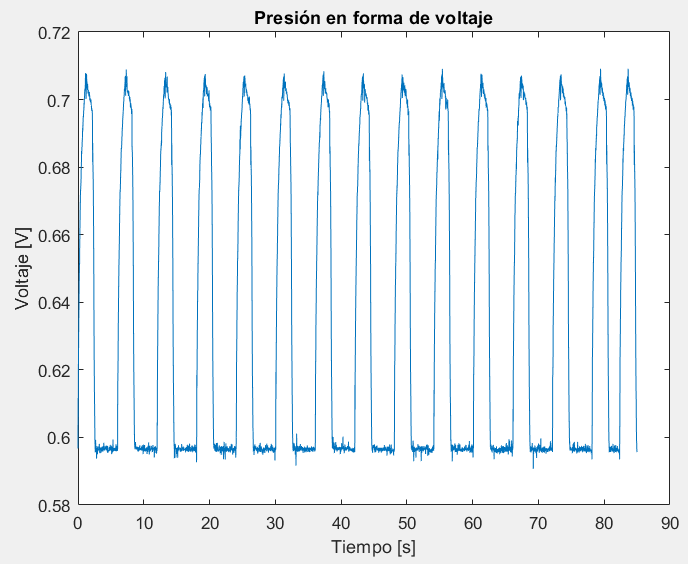
\includegraphics[width=0.4\textwidth]{media/presion-voltaje}
		\caption{Presión en forma de voltaje}
		\label{fig:presion-voltaje}
	\end{figure}
	
	Luego después de procesar cada dato mediante la recta calculada en \ref{eq:calibracion-presion} se obtuvieron los datos de presión en [cmH20] y cuya gráfica se muestra en la figura \ref{fig:presion}
	
	\begin{figure}[h]
		\centering
		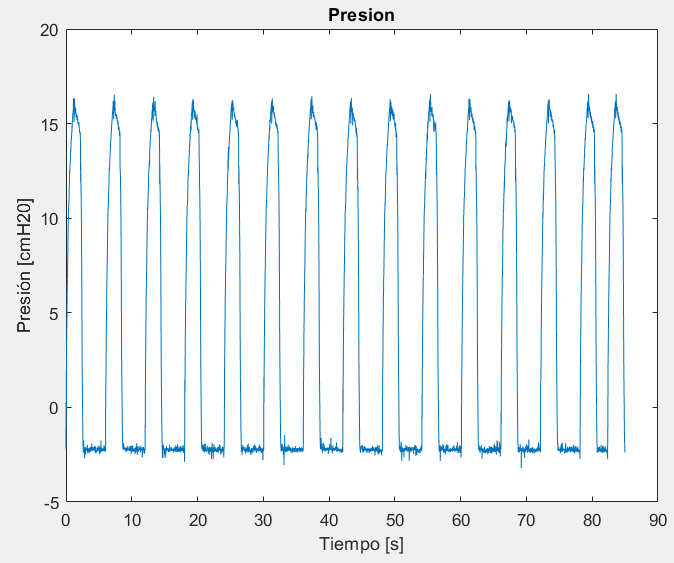
\includegraphics[width=0.4\textwidth]{media/presion}
		\caption{Presión expresada en cm de agua}
		\label{fig:presion}
	\end{figure}
	
	\section{Calculo del volumen en un semiciclo}
	
	Al analizar de forma detenida la gráfica mostrada en \ref{fig:flujo} se determina el tiempo para un semiciclo de la señal, estando el ultimo punto digital en 1.24s como se muestra gráficamente en \ref{fig:semiciclo-flujo} 
	
	\begin{figure}[h]
		\centering
		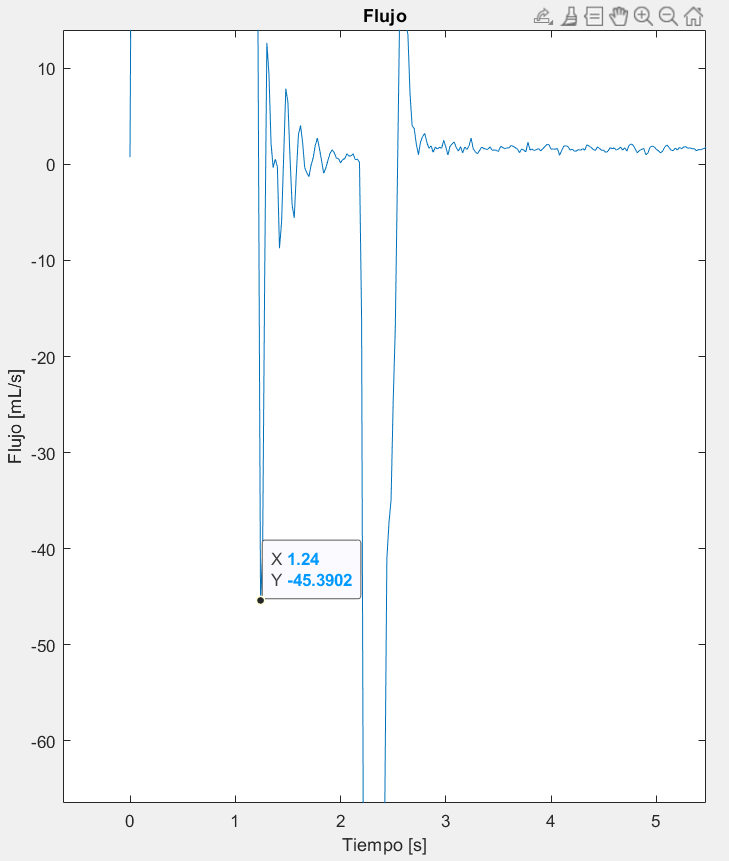
\includegraphics[width=0.4\textwidth]{media/semiciclo-flujo}
		\caption{Primer semiciclo del Flujo en mL/s}
		\label{fig:semiciclo-flujo}
	\end{figure}
	
	Una vez definido el tiempo de inspiración (primer semiciclo) es posible determinar el volumen al integrar la señal en el intervalo [0, 1.24], como se define en la ecuación \ref{eq:volumen}
	
	\begin{equation}
		V = \int_{t_1}^{t_2}{f(t)dt}
		\label{eq:volumen}
	\end{equation}
	
	Donde f(t) representa la función de flujo en el dominio del tiempo, al aplicar este procedimiento en MATLAB el volumen obtenido es $V = 56.7277 m^3$.
	
	\section{Código MATLAB}
	
	El código MATLAB para ambos casos flujo y presión se muestran en los bloques de código \ref{lst:flujo} y \ref{lst:presion} respectivamente.
	
	\begin{lstlisting}[numbers=none, caption="Análisis de flujo vs Voltaje", label=lst:flujo]
		
		clc, clear, close all;
		
		% Importar los datos
		data = load("flujo.txt");
		
		Ts = 0.02;
		Fs = 1/Ts;
		
		t = 0 : Ts : length(data)/Fs - Ts;
		
		% Relacion entre voltaje y flujo (mediante la hoja de datos del ventilador)
		
		flujo(1) = 0;
		for i = 1 : length(data)
		flujo(i) = 5*(data(i) - 1)*1000/60;
		end
		
		% Obtencion del volumen
		volumen = trapz(t(1:62), flujo(1:62));
		disp(volumen);
		
		figure;
		subplot(1, 2, 1);
		plot(t, data);
		title("Flujo expresado en Voltaje");
		xlabel("Tiempo [s]");
		ylabel("Voltaje [V]");
		
		subplot(1, 2, 2);
		plot(t, flujo);
		title("Flujo");
		xlabel("Tiempo [s]"),
		ylabel("Flujo [mL/s]");
		
		
		figure
		plot(flujo, data);
		title("Voltaje - Flujo de aire");
		xlabel("Flujo [mL/s]");
		ylabel("Voltaje [V]");
		
	\end{lstlisting}	
	
	\begin{lstlisting}[numbers=none, caption="Análisis presión - Voljate", label=lst:presion]
		clc, clear, close all;
		% Obtencion de los datos
		data = load("presion.txt");
		
		Ts = 0.02;
		Fs = 1/Ts;
		
		t = 0 : Ts : length(data)/Fs - Ts;
		
		presion(1) = 0;
		
		for i = 1 : length(data)
		presion(i) = 167*data(i) - 101.85;
		end
		
		subplot(1, 2, 1);
		plot(t, data);
		title("Presion en forma de voltaje");
		xlabel("Tiempo [s]");
		ylabel("Voltaje [V]");
		
		subplot(1, 2, 2);
		plot(t, presion);
		title("Presion");
		xlabel("Tiempo [s]");
		ylabel("Presion [cmH20]");
	\end{lstlisting}
	
	\bibliographystyle{IEEEtran}
	\bibliography{biblio}
\end{document}
